% ----------------------------------------------------------------------------------------------------- %
% Relatório 4 de PDS - Baseado na classe UFTeX
% ----------------------------------------------------------------------------------------------------- %

\documentclass[tcc]{classe_uftex/uftex}
% ---- Esse comando cria o nome uftex estilizado
\newcommand\uftex{UF\TeX}

\usepackage{lipsum}
\usepackage{tikz}
\usepackage[siunitx]{circuitikz}
\usetikzlibrary{arrows}

\usepackage[alf,abnt-emphasize=bf]{referencias_abnt/abntex2cite}
\usepackage{amsmath}
\usepackage{xcolor}
\usepackage{mathptmx} % Times New Roman (ABNT)
\usepackage{float}

\renewcommand{\lstlistingname}{Código}
\renewcommand{\lstlistlistingname}{Lista de Códigos}

\definecolor{codegreen}{rgb}{0,0.6,0}
\definecolor{codegray}{rgb}{0.5,0.5,0.5}
\definecolor{codepurple}{rgb}{0.58,0,0.82}
\definecolor{backcolour}{rgb}{0.98,0.98,0.98}
\definecolor{codeblue}{rgb}{0,0,0.8}

\lstset{
  language=Matlab,
  backgroundcolor=\color{backcolour},
  commentstyle=\color{codegreen},
  keywordstyle=\color{codeblue}\bfseries,
  numberstyle=\normalsize\color{codegray},
  stringstyle=\color{codepurple},
  basicstyle=\ttfamily\small\color{black},
  breakatwhitespace=false,
  breaklines=true,
  captionpos=b,
  keepspaces=true,
  numbers=left,
  numbersep=12pt,
  showspaces=false,
  showstringspaces=false,
  showtabs=false,
  tabsize=2,
  frame=lines,
  rulecolor=\color{black!30},
  xleftmargin=20pt,
  framexleftmargin=5pt,
  aboveskip=20pt,
  belowskip=20pt
}

\renewcommand{\backrefpagesname}{}
\renewcommand{\backref}{}
\renewcommand*{\backrefalt}[4]{}

% ---- Ajuste para transformar a capa de TCC em Relatório e numeração no rodapé
\makeatletter
\renewcommand*{\ps@plain}{%
  \let\@mkboth\@gobbletwo
  \let\@oddhead\@empty
  \def\@oddfoot{%
    \reset@font
    \hfil
    \thepage
  }%
  \let\@evenhead\@empty
  \let\@evenfoot\@oddfoot
}

\renewcommand\frontpage@maintext{
  \sloppy\nohyphens{Relatório de Laboratório apresentado à disciplina de Processamento Digital de Sinais do curso de \local@deptname\ da \local@universityname .

 \vspace{.5cm}
  \nohyphens{%
    \count1=0
    \@whilenum \count1<\@advisor \do{%
    \ifcase\count1 % same as \ifnum0=\count1
        Professor: \csname uftAdvisorDegree:\the\count1 \endcsname \
        \csname uftAdvisorName:\the\count1 \endcsname \
        \csname uftAdvisorSurname:\the\count1 \endcsname \ \par
    \else
        \local@coadvisorstring: \csname uftAdvisorDegree:\the\count1 \endcsname \
        \csname uftAdvisorName:\the\count1 \endcsname \
        \csname uftAdvisorSurname:\the\count1 \endcsname \ \par
    \fi
    \advance\count1 by 1}
  } \par
}
}
\makeatother

% ---- Início do documento
\begin{document}
  % ---- Descrição do título do trabalho
  \title{Relatório 4 de PDS: Transformada de Fourier em Tempo Discreto}
  % ---- Nome do autor ou autores do trabalho
  \author{Maurício}{Moura de Carvalho}
  % ---- Nome do orientador do trabalho.
  \advisor{Prof.}{Ivan}{Ney Alvizuri Romani}{Dr.}

  % ---- Departamento
  \department{EE}

  % ---- Data
  \date{08}{06}{2026}

  % ---- Palavras-chaves
  \keyword{Processamento Digital de Sinais}
  \keyword{Transformada de Fourier em Tempo Discreto}
  \keyword{Octave}

  % ---- Palavras-chaves em inglês
  \foreignkeyword{Digital Signal Processing}
  \foreignkeyword{Discrete-Time Fourier Transform}
  \foreignkeyword{Octave}

  \maketitle
  \frontmatter

  % ---- Cria o sumário
  \tableofcontents

  % --- Marca o inicio dos elementos textuais
  \mainmatter
  \setcounter{page}{1}
  \onehalfspacing

% ----------------------------------------------------------------------------------------------------- %
% Capítulos do trabalho
% ----------------------------------------------------------------------------------------------------- %

\chapter{Introdução}

Este relatório apresenta os resultados do quarto laboratório da disciplina de Processamento Digital de Sinais (PDS), dedicado ao tema da \textbf{Transformada de Fourier em Tempo Discreto (TFTD)}. A TFTD é uma ferramenta central na análise de sistemas e sinais discretos, pois permite representar qualquer sequência no domínio da frequência, revelando seu conteúdo espectral de forma precisa.

Ao contrário da Transformada Discreta de Fourier (DFT), a TFTD opera sobre sequências de duração finita ou infinita e produz um espectro contínuo e periódico em frequência com período $2\pi$. Esta periodicidade é uma consequência direta da natureza discreta das amostras e constitui uma das propriedades mais importantes do domínio da frequência em tempo discreto.

O objetivo desta prática foi calcular analiticamente e verificar numericamente a TFTD de diferentes sinais, investigar a periodicidade do espectro e verificar graficamente a propriedade de deslocamento em frequência. As implementações foram realizadas no ambiente Octave \cite{octaveman}, seguindo o roteiro de laboratório \cite{roteiro04} e com suporte nas referências de Proakis e Manolakis \cite{proakis_manolakis} e Ingle \cite{ingle2017}.

\chapter{Metodologia e Procedimentos Práticos}

\section{Parte I -- TFTD de $x[n] = (0{,}5)^n u[n]$}

A TFTD de uma sequência $x[n]$ é definida como:
\begin{equation}
  X(e^{j\omega}) = \sum_{n=-\infty}^{+\infty} x[n]\, e^{-j\omega n}
  \label{eq:tftd_def}
\end{equation}

Para $x[n] = (0{,}5)^n u[n]$, a soma começa em $n=0$ e a série geométrica converge pois $|0{,}5| < 1$:
\begin{equation}
  X(e^{j\omega}) = \sum_{n=0}^{\infty} (0{,}5)^n e^{-j\omega n}
  = \sum_{n=0}^{\infty} \left(0{,}5\, e^{-j\omega}\right)^n
  = \frac{1}{1 - 0{,}5\, e^{-j\omega}}
  \label{eq:tftd_parte1}
\end{equation}

A expressão em forma fechada \eqref{eq:tftd_parte1} foi avaliada numericamente em 501 pontos equidistantes no intervalo $[0, \pi]$, e foram plotadas a magnitude $|X(e^{j\omega})|$, o ângulo $\angle X(e^{j\omega})$, a parte real e a parte imaginária.

\section{Parte II -- TFTD de $x[n] = \{1, 2, 3, 4, 5\}$}

Para a sequência finita $x[n] = \{1, 2, 3, 4, 5\}$ definida para $0 \leq n \leq 4$, a TFTD é uma soma finita:
\begin{equation}
  X(e^{j\omega}) = \sum_{n=0}^{4} x[n]\, e^{-j\omega n}
  = 1 + 2e^{-j\omega} + 3e^{-j2\omega} + 4e^{-j3\omega} + 5e^{-j4\omega}
  \label{eq:tftd_parte2}
\end{equation}

A avaliação numérica foi feita em 501 frequências equidistantes entre $[0, \pi]$, com plotagem das quatro representações espectrais.

\section{Parte III -- TFTD de $x[n] = (0{,}9\,e^{j\pi/3})^n$, $0 \leq n \leq 10$}

A sequência complexa $x[n] = (0{,}9\,e^{j\pi/3})^n = (0{,}9)^n e^{j\frac{\pi}{3}n}$ tem suporte finito $0 \leq n \leq 10$. Sua TFTD é:
\begin{equation}
  X(e^{j\omega}) = \sum_{n=0}^{10} (0{,}9)^n e^{j\frac{\pi}{3}n}\, e^{-j\omega n}
  = \sum_{n=0}^{10} (0{,}9)^n\, e^{j\left(\frac{\pi}{3} - \omega\right)n}
  \label{eq:tftd_parte3}
\end{equation}

O espectro foi avaliado no intervalo $[-2\pi, 2\pi]$ para evidenciar a \textbf{periodicidade} de $2\pi$ da TFTD, propriedade universal decorrente do caráter discreto das amostras: $X(e^{j(\omega + 2\pi k)}) = X(e^{j\omega})$ para qualquer inteiro $k$.

\section{Parte IV -- Propriedade de Deslocamento em Frequência}

A propriedade de deslocamento em frequência da TFTD afirma que, se $Y(e^{j\omega})$ é a TFTD de $y[n] = e^{j\omega_0 n} x[n]$, então:
\begin{equation}
  Y(e^{j\omega}) = X(e^{j(\omega - \omega_0)})
  \label{eq:freq_shift}
\end{equation}

Para verificar essa propriedade, utilizaram-se:
\begin{itemize}
  \item $x[n] = \cos\!\left(\frac{\pi n}{2}\right)$, $0 \leq n \leq 10$
  \item $y[n] = e^{j\frac{\pi}{4}n}\, x[n]$, com $\omega_0 = \pi/4$
\end{itemize}
Segundo a propriedade \eqref{eq:freq_shift}, espera-se que o espectro de $y[n]$ seja o espectro de $x[n]$ deslocado de $\pi/4$ em direção a frequências mais altas. Ambas as TFTDs foram calculadas numericamente em 1001 pontos no intervalo $[-\pi, \pi]$ e comparadas graficamente.

\chapter{Resultados e Discussões}

\section{Parte I: Sinal Exponencial Real de Duração Infinita}

A forma fechada $X(e^{j\omega}) = 1/(1 - 0{,}5\,e^{-j\omega})$ foi avaliada diretamente, aproveitando que a expressão analítica é conhecida. O Código~1 implementa o cálculo e gera os quatro gráficos.

\lstinputlisting[language=Matlab, caption={{Script para a Parte I.}}]{codigos/parte1.m}

O script cria um vetor de 501 frequências equidistantes em $[0, \pi]$ e avalia a forma fechada da TFTD de forma vetorizada, aproveitando os operadores elemento a elemento do Octave (\texttt{./} e \texttt{exp}). Em seguida, organiza a figura em uma grade $2\times2$ de subplots, plotando em cada painel uma representação distinta do espectro: magnitude (\texttt{abs}), fase (\texttt{angle}), parte real (\texttt{real}) e parte imaginária (\texttt{imag}), todas em função da frequência normalizada $\omega/\pi$. A figura é salva com \texttt{saveas}.

\begin{figure}[H]
\centering

\includegraphics[width=0.95\textwidth]{figuras/parte1.png}
\caption{TFTD de $x[n]=(0{,}5)^n u[n]$: magnitude, fase, parte real e imaginária.}\label{fig:p1}
\end{figure}

\textbf{Magnitude.} O espectro $|X(e^{j\omega})|$ exibe comportamento de filtro passa-baixas: seu valor máximo ocorre em $\omega = 0$, onde $|X(e^{j0})| = 1/(1-0{,}5) = 2$, e seu valor mínimo em $\omega = \pi$, onde $|X(e^{j\pi})| = 1/(1+0{,}5) = 1/1{,}5 \approx 0{,}667$. A razão física é que, em $\omega = 0$, todas as amostras da sequência (que decaem positivamente) somam-se em fase; em $\omega = \pi$, os termos alternam de sinal e se cancelam parcialmente. A expressão exata é:
\begin{equation}
  |X(e^{j\omega})| = \frac{1}{\sqrt{(1-0{,}5\cos\omega)^2 + (0{,}5\sin\omega)^2}}
  = \frac{1}{\sqrt{1{,}25 - \cos\omega}} \nonumber
\end{equation}

\textbf{Fase.} A fase é dada por $\angle X(e^{j\omega}) = -\arctan\!\left(\dfrac{0{,}5\sin\omega}{1-0{,}5\cos\omega}\right)$. Em $\omega = 0$ e $\omega = \pi$ a parte imaginária do denominador é nula, portanto $\angle X = 0$ em ambos os extremos. A fase atinge seu valor mais negativo em $\omega = \pi/3$ ($\omega/\pi \approx 0{,}33$), onde $\angle X = -\arctan\!\left(\frac{0{,}5\sin(\pi/3)}{1-0{,}5\cos(\pi/3)}\right) = -\pi/6 \approx -0{,}52\,\text{rad}$, e retorna a zero em $\omega = \pi$. O comportamento não é linear porque o sistema possui um polo em $z = 0{,}5$ (fase não linear é esperada para sistemas com polos não nulos).

\textbf{Parte real.} $\text{Re}\{X(e^{j\omega})\} = (1-0{,}5\cos\omega)/(1{,}25 - \cos\omega)$. Como o numerador e denominador são ambos positivos para todo $\omega \in [0,\pi]$, a parte real é sempre positiva, decrescendo de $2$ em $\omega=0$ até $0{,}667$ em $\omega=\pi$. A parte real domina a magnitude neste caso, o que é condizente com a natureza real e positiva de $x[n]$.

\textbf{Parte imaginária.} $\text{Im}\{X(e^{j\omega})\} = -0{,}5\sin\omega/(1{,}25 - \cos\omega)$. É identicamente zero em $\omega = 0$ e $\omega = \pi$ (onde $\sin\omega = 0$) e atinge seu valor mais negativo onde $\cos\omega = 0{,}8$, ou seja, em $\omega \approx 0{,}64\,\text{rad}$ ($\omega/\pi \approx 0{,}2$), valendo $\text{Im}\{X\} = -0{,}5 \cdot 0{,}6/0{,}45 = -2/3 \approx -0{,}667$. O sinal negativo decorre da causalidade do sistema: uma sequência que começa em $n=0$ e decai para $n>0$ concentra energia no semiplano imaginário negativo do espectro, resultado direto do sinal negativo de $e^{-j\omega n}$ na definição da TFTD.

% ------------------------------------------------------------------ %
\section{Parte II: Sequência Finita $\{1, 2, 3, 4, 5\}$}

Por tratar-se de uma soma finita, a TFTD foi calculada diretamente pela definição \eqref{eq:tftd_parte2}, sem qualquer aproximação. O Código~2 implementa o cálculo iterando sobre cada ponto de frequência.

\lstinputlisting[language=Matlab, caption={{Script para a Parte II.}}]{codigos/parte2.m}

O script define a sequência \texttt{x = [1 2 3 4 5]} e seu vetor de índices \texttt{n = 0:4}, além de 501 pontos de frequência em $[0, \pi]$. Como não há forma fechada simples, a TFTD é calculada pela definição via laço \texttt{for}: em cada iteração $k$, a expressão \texttt{sum(x .* exp(-1j * w(k) * n))} realiza o somatório $\sum_{n=0}^{4} x[n]\,e^{-j\omega_k n}$ de forma vetorial. O vetor resultado \texttt{X} é pré-alocado com \texttt{zeros} para eficiência. A estrutura gráfica de quatro subplots é idêntica à Parte I.

\begin{figure}[H]
\centering
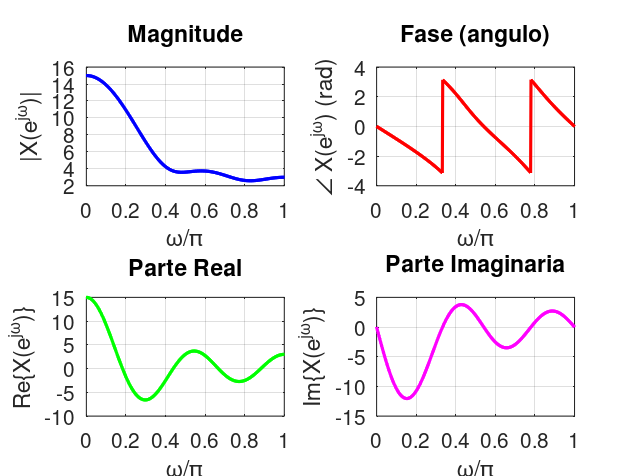
\includegraphics[width=0.95\textwidth]{figuras/parte2.png}
\caption{TFTD de $x[n]=\{1,2,3,4,5\}$: magnitude, fase, parte real e imaginária.}\label{fig:p2}
\end{figure}

\textbf{Magnitude.} O valor máximo da magnitude ocorre em $\omega = 0$, onde todos os termos da soma se somam construtivamente: $X(e^{j0}) = 1+2+3+4+5 = 15$. Em $\omega = \pi$, os termos alternam de sinal e a soma resulta em $X(e^{j\pi}) = 1-2+3-4+5 = 3$, que é o valor mínimo no intervalo. O espectro exibe lóbulos secundários de amplitude decrescente entre $\omega = 0$ e $\omega = \pi$, com zeros intermediários que dependem da estrutura polinomial da TFTD: $X(e^{j\omega}) = 1 + 2e^{-j\omega} + 3e^{-j2\omega} + 4e^{-j3\omega} + 5e^{-j4\omega}$, que é um polinômio de grau 4 em $e^{-j\omega}$.

\textbf{Fase.} Como $x[n]$ é uma sequência \emph{real}, a TFTD satisfaz simetria conjugada: $X(e^{-j\omega}) = X^*(e^{j\omega})$. Isso implica que a magnitude é par e a fase é ímpar em $\omega$. No intervalo $[0, \pi]$, a fase é nula em $\omega = 0$ (onde $X$ é real e positiva, valendo 15) e em $\omega = \pi$ (onde $X$ é real e positiva, valendo 3). A fase não é linear porque a sequência $\{1,2,3,4,5\}$ não é \emph{simétrica} (palíndroma): se fosse do tipo $\{a,b,c,b,a\}$, a fase seria exatamente linear, característica de filtros FIR de fase linear. A assimetria dos coeficientes impõe variações não lineares na fase entre os dois extremos.

\textbf{Parte real.} Como $x[n]$ é real, $\text{Re}\{X(e^{j\omega})\} = \sum_{n=0}^{4} x[n]\cos(\omega n)$ é uma função \emph{par} de $\omega$. Em $\omega = 0$ assume o valor 15 e vai oscilando, podendo ser negativa em certas frequências onde os cossenos ponderados pelos coeficientes crescentes resultam em soma negativa.

\textbf{Parte imaginária.} Analogamente, $\text{Im}\{X(e^{j\omega})\} = -\sum_{n=0}^{4} x[n]\sin(\omega n)$ é \emph{ímpar} em $\omega$, portanto nula em $\omega=0$ e em $\omega=\pi$ (onde $\sin(\pi n) = 0$ para todo inteiro $n$). O fato de que a parte imaginária é não nula entre esses extremos é consequência direta da não-simetria da sequência: coeficientes assimétricos geram contribuições senoidais que não se cancelam.

% ------------------------------------------------------------------ %
\section{Parte III: Periodicidade da TFTD}

O espectro foi calculado no intervalo estendido $[-2\pi, 2\pi]$ para evidenciar a periodicidade de $2\pi$.

\lstinputlisting[language=Matlab, caption={{Script para a Parte III.}}]{codigos/parte3.m}

O script define a sequência complexa $x[n] = (0{,}9\,e^{j\pi/3})^n$ para $n = 0, \ldots, 10$ e calcula sua TFTD numericamente pela definição em 2001 pontos de frequência distribuídos em $[-2\pi, 2\pi]$ — intervalo propositalmente duas vezes mais largo que o período fundamental, para expor dois ciclos completos do espectro. O laço \texttt{for} segue a mesma estrutura da Parte II. Na plotagem, linhas verticais tracejadas em múltiplos inteiros de $\pi$ e marcações de eixo a cada $0{,}5\,\pi$ destacam visualmente as fronteiras entre períodos, facilitando a verificação da periodicidade tanto na magnitude quanto na fase.

\begin{figure}[H]
\centering
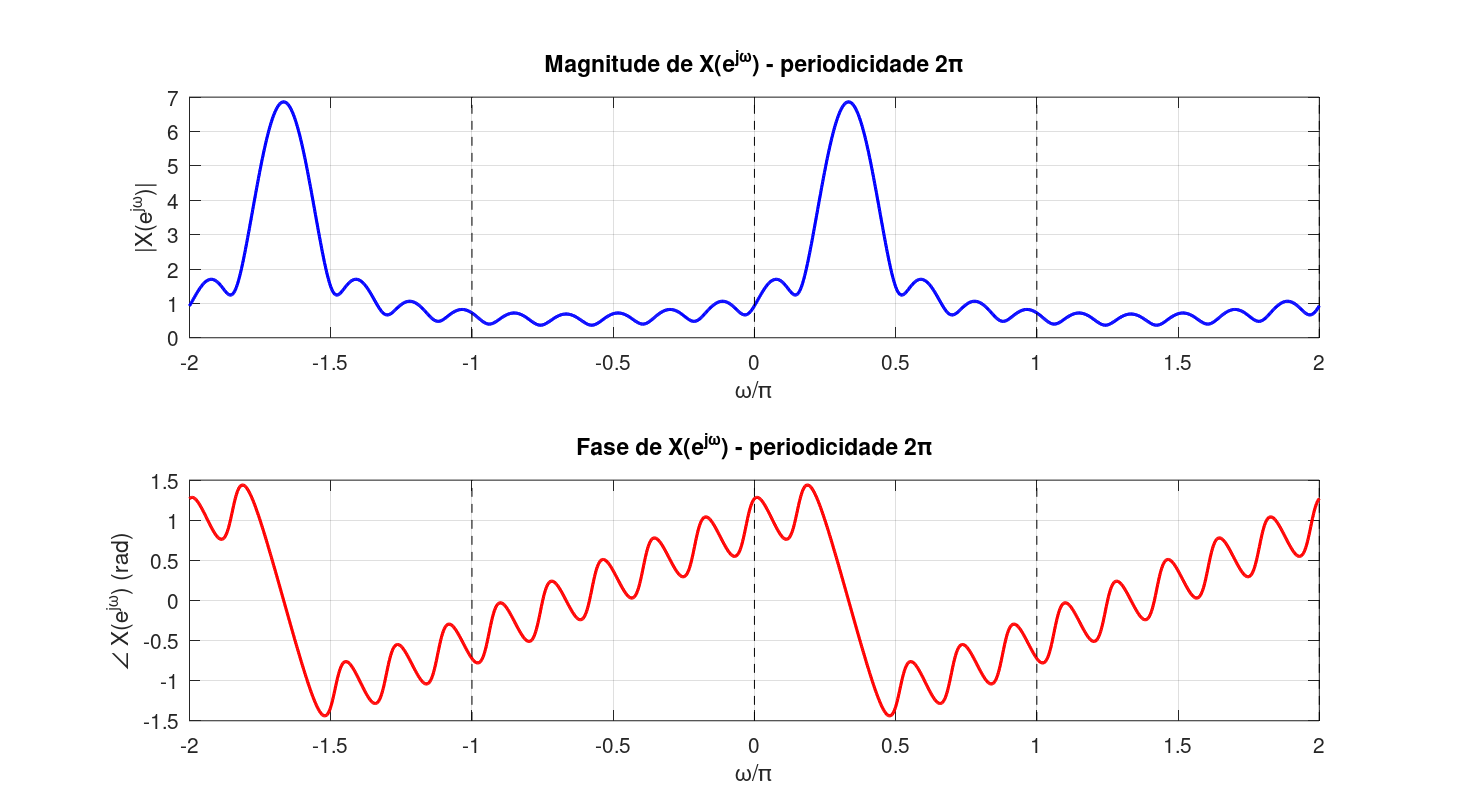
\includegraphics[width=0.95\textwidth]{figuras/parte3.png}
\caption{TFTD de $x[n]=(0{,}9\,e^{j\pi/3})^n$: periodicidade $2\pi$ da magnitude e da fase.}\label{fig:p3}
\end{figure}

\textbf{Periodicidade.} Os gráficos confirmam diretamente que $X(e^{j(\omega+2\pi)}) = X(e^{j\omega})$ para todo $\omega$. A prova matemática decorre da definição: substituindo $\omega + 2\pi$ na equação \eqref{eq:tftd_def} e usando o fato de que $e^{-j2\pi n} = 1$ para qualquer inteiro $n$,
\begin{equation}
  X\!\left(e^{j(\omega+2\pi)}\right) = \sum_{n=0}^{10} x[n]\,e^{-j(\omega+2\pi)n}
  = \sum_{n=0}^{10} x[n]\,e^{-j\omega n}\underbrace{e^{-j2\pi n}}_{=\,1}
  = X(e^{j\omega}) \nonumber
\end{equation}
As linhas verticais tracejadas em $\omega/\pi = -2, -1, 0, 1, 2$ delimitam os períodos e tornam visível a repetição idêntica do padrão.

\textbf{Posição e forma do pico.} O pico de magnitude ocorre em $\omega = \pi/3$ ($\omega/\pi = 1/3 \approx 0{,}333$), exatamente na frequência angular da exponencial complexa $e^{j\pi n/3}$ embutida na sequência. Para uma sequência infinita $(0{,}9)^n e^{j\pi n/3} u[n]$, a TFTD seria $1/\bigl(1-0{,}9\,e^{j(\pi/3-\omega)}\bigr)$ — um pico infinitamente agudo (polo). Com apenas 11 amostras, o pico tem largura finita (alargamento espectral), pois a janela retangular de duração $N=11$ convolui o espectro com uma função do tipo $\text{Dirichlet}(N,\omega)$, introduzindo lóbulos laterais visíveis.

\textbf{Ausência de simetria conjugada.} Como $x[n]$ é uma sequência \emph{complexa}, a TFTD \textbf{não} satisfaz simetria conjugada. Isso é evidente nos gráficos: o pico de magnitude aparece \emph{somente} em $\omega = \pi/3$, sem réplica em $\omega = -\pi/3$. Se $x[n]$ fosse real, o espectro seria par e haveriam picos simétricos em $\pm\pi/3$. A natureza complexa de $x[n]$ quebra essa simetria, sendo essa uma distinção fundamental entre sinais reais e complexos no domínio da frequência.

\textbf{Fase.} O gráfico de fase confirma a mesma periodicidade de $2\pi$. A fase varia de forma não linear em torno do pico em $\omega = \pi/3$, apresentando transições abruptas próximas aos zeros do espectro, onde a fase salta de $+\pi$ para $-\pi$ (descontinuidades de $2\pi$ introduzidas pela função \texttt{angle()}, que retorna valores no intervalo $(-\pi, \pi]$).

% ------------------------------------------------------------------ %
\section{Parte IV: Deslocamento em Frequência}

\lstinputlisting[language=Matlab, caption={{Script para a Parte IV.}}]{codigos/parte4.m}

O script define $x[n] = \cos(\pi n/2)$ e $y[n] = e^{j\pi n/4}\,x[n]$ para $n = 0, \ldots, 10$, sendo $y[n]$ a versão de $x[n]$ modulada por uma exponencial complexa de frequência $\omega_0 = \pi/4$. Um único laço \texttt{for} sobre 1001 pontos em $[-\pi, \pi]$ computa as TFTDs de ambos os sinais simultaneamente pela definição. Os resultados são dispostos em grade 2$\times$2: magnitude e fase de $X(e^{j\omega})$ na coluna da esquerda (azul) e de $Y(e^{j\omega})$ na coluna da direita (vermelho), permitindo comparação visual direta do deslocamento espectral.

\begin{figure}[H]
\centering

\includegraphics[width=0.95\textwidth]{figuras/parte4.png}
\caption{Verificação da propriedade de deslocamento em frequência: magnitude e fase de $X(e^{j\omega})$ e $Y(e^{j\omega})$.}\label{fig:p4}
\end{figure}

\textbf{Espectro de $x[n]$ (magnitude).} O cosseno pode ser decomposto via Euler: $\cos(\pi n/2) = \frac{1}{2}e^{j\pi n/2} + \frac{1}{2}e^{-j\pi n/2}$. Sendo $x[n]$ real e de suporte finito, sua TFTD concentra energia nas frequências $\omega = \pm\pi/2$. No intervalo $[-\pi, \pi]$ exibido, o gráfico de $|X(e^{j\omega})|$ apresenta dois picos simétricos em $\omega/\pi = +0{,}5$ e $\omega/\pi = -0{,}5$. A simetria par da magnitude é garantida pela natureza real de $x[n]$: como $X(e^{-j\omega}) = X^*(e^{j\omega})$, segue-se que $|X(e^{-j\omega})| = |X(e^{j\omega})|$.

\textbf{Espectro de $y[n]$ (magnitude).} Após a modulação por $e^{j\pi n/4}$ ($\omega_0 = \pi/4$), a propriedade \eqref{eq:freq_shift} prevê $Y(e^{j\omega}) = X(e^{j(\omega - \pi/4)})$. Os picos que estavam em $\omega = \pm\pi/2$ deslocam-se de $+\pi/4$, resultando em:
\begin{itemize}
  \item Pico em $\omega = +\pi/2 + \pi/4 = +3\pi/4$ ($\omega/\pi = +0{,}75$)
  \item Pico em $\omega = -\pi/2 + \pi/4 = -\pi/4$ ($\omega/\pi = -0{,}25$)
\end{itemize}
O gráfico de $|Y(e^{j\omega})|$ confirma exatamente essas posições. Nota-se que a magnitude de $Y$ \textbf{não é simétrica} em torno de $\omega = 0$: os dois picos, embora de mesma amplitude, estão em posições assimétricas ($-0{,}25\pi$ e $+0{,}75\pi$). Isso ocorre porque $y[n]$ é uma sequência \emph{complexa} (produto de um real por um complexo), e sequências complexas não satisfazem simetria conjugada — a condição $Y(e^{-j\omega}) = Y^*(e^{j\omega})$ só vale para sequências reais.

\textbf{Fase de $x[n]$.} Como $x[n]$ é real, $\angle X(e^{j\omega})$ é uma função ímpar de $\omega$. O gráfico exibe transições abruptas de fase nos picos espectrais (onde a magnitude tende a zero entre os lóbulos), reflexo do comportamento da função \texttt{angle()} que restringe os valores ao intervalo $(-\pi, \pi]$.

\textbf{Fase de $y[n]$.} A fase de $Y(e^{j\omega}) = X(e^{j(\omega-\pi/4)})$ é a fase de $X$ avaliada em $(\omega-\pi/4)$, portanto é a fase de $X$ \emph{transladada} em $\pi/4$ para a direita no eixo de frequência. O gráfico confirma essa relação: o padrão de fase de $Y$ reproduz o de $X$, porém deslocado, e não é mais uma função ímpar de $\omega$ (pois $y[n]$ é complexo), o que é visualmente evidente na assimetria do gráfico em relação à origem.

\chapter{Conclusão}

Este laboratório consolidou o estudo da Transformada de Fourier em Tempo Discreto (TFTD) em suas dimensões analítica e computacional. Através das quatro atividades realizadas, foi possível:

\begin{itemize}
  \item Calcular analiticamente a TFTD de uma exponencial real de duração infinita, explorando a convergência da série geométrica e identificando o comportamento de filtragem passa-baixas inerente a um polo próximo à origem.
  \item Avaliar numericamente a TFTD de uma sequência finita de curto comprimento, verificando que em $\omega = 0$ o resultado corresponde à soma de todos os coeficientes.
  \item Confirmar experimentalmente que a TFTD é sempre $2\pi$-periódica em frequência, propriedade universal decorrente da natureza amostrada dos sinais discretos.
  \item Verificar graficamente a propriedade de deslocamento em frequência, observando que a multiplicação por uma exponencial complexa $e^{j\omega_0 n}$ no domínio do tempo equivale a uma translação $\omega_0$ no espectro de frequência.
\end{itemize}

O Octave \cite{octaveman} demonstrou-se uma plataforma adequada para a investigação numérica desses conceitos, permitindo a avaliação da TFTD em um número arbitrário de pontos de frequência e a visualização simultânea de magnitude, fase, parte real e imaginária. Os resultados obtidos estão em plena concordância com a teoria apresentada por Proakis e Manolakis \cite{proakis_manolakis} e Ingle \cite{ingle2017}.

% ----------------------------------------------------------------------------------------------------- %
\backmatter
\singlespacing
% ----------------------------------------------------------------------------------------------------- %
\bibliography{relatorio_4}

\end{document}
